%\subsection{Benchmark}
%
%\begin{frame}
%    Comparaison des performances (latence, débit) entre SQL et NoSQL sur des cas d’usage.
%    Exemple : Benchmark MongoDB vs PostgreSQL pour des requêtes de type "find all users with age > 25".
%    Outils : Utiliser des données réelles (ex : TechEmpower Benchmarks).
%\end{frame}

\begin{frame}{Avantages et inconvénients du NoSQL}

    \pause

    \prosbox{
    \textbf{Avantages}
    \begin{itemize}
        \item Flexibilité du schéma
        \item Scalabilité horizontale
    \end{itemize}
    }

    \note{

        Flexibilité du schéma : pas de structure rigide, adapté aux données non structurées ou évolutives (JSON, documents, graphes...)

        Scalabilité horizontale : conçu pour répartir la charge sur plusieurs serveurs facilement, idéal pour les gros volumes de données

    }

    \vspace{0.5cm}
    \pause

    \consbox{
    \textbf{Inconvénients}
    \begin{itemize}
        \item Consistance limitée
        \item Écosystème et requêtes moins matures
    \end{itemize}
    }

    \note
    {
        Cohérence limitée : privilégie souvent la disponibilité à la cohérence forte (modèle BASE plutôt qu'ACID), ce qui peut poser problème pour les transactions critiques + théorème CAP

        Écosystème et requêtes moins matures : pas de langage standard comme SQL, jointures complexes difficiles, et moins d'outils/expertise disponibles selon la technologie choisie
    }

\end{frame}

\begin{frame}{Quand utiliser une base NoSQL ?}

    \begin{figure}[htb]
        \centering
        \resizebox{\textwidth}{!}{
        \begin{tikzpicture}

            \node[inner sep=0pt, label=below:Big Data] (big-data) at (0,0)
                {\includegraphics[width=.2\textwidth]{img/icon/big-data.png}};

            \node[inner sep=0pt, label=below:Temps réel, right=of big-data, xshift=1cm] (real-time)
                {\includegraphics[width=.2\textwidth]{img/icon/real-time.png}};

            \node[inner sep=0pt, label=below:Données non-structurées, right=of real-time, xshift=1cm] (unstructured)
                {
\includegraphics[width=.2\textwidth]{img/icon/unstructured.png}};
        \end{tikzpicture}
        }
    \end{figure}

    \note{
        À noter que le choix dépend surtout du cas d'usage : NoSQL brille pour le Big Data, le temps réel ou les données semi-structurées, alors que SQL reste préférable pour les données fortement relationnelles nécessitant des garanties transactionnelles strictes.

        \begin{itemize}
            \item Grande quantité de données semi-structurées ou non structurées (logs, réseaux sociaux, IoT, time-based data)
            \item Améliorer les performances d'accès aux données en combinant le traitement de volumes de données plus importants, la réduction des temps de latence et l'amélioration du débit.
        \end{itemize}

        Quelques exemples d'applications qui bénéficient de l'utilisation de bases NoSQL :
        \begin{itemize}
            \item Applications web et mobiles
            \item Big Data et analytics
            \item Gestion de contenu et réseaux sociaux
            \item Internet des objets (IoT)
        \end{itemize}
    }

\end{frame}

\begin{frame}{SQL vs NoSQL expliqué en 4 minutes}
    \centering
    % SQL vs. NoSQL Explained (in 4 Minutes): https://www.youtube.com/watch?v=_Ss42Vb1SU4
    \href{run:/Users/alanna/Documents/Teaching/2026-2027/IUT/NoSQL/Cours/video/nosql.mp4}{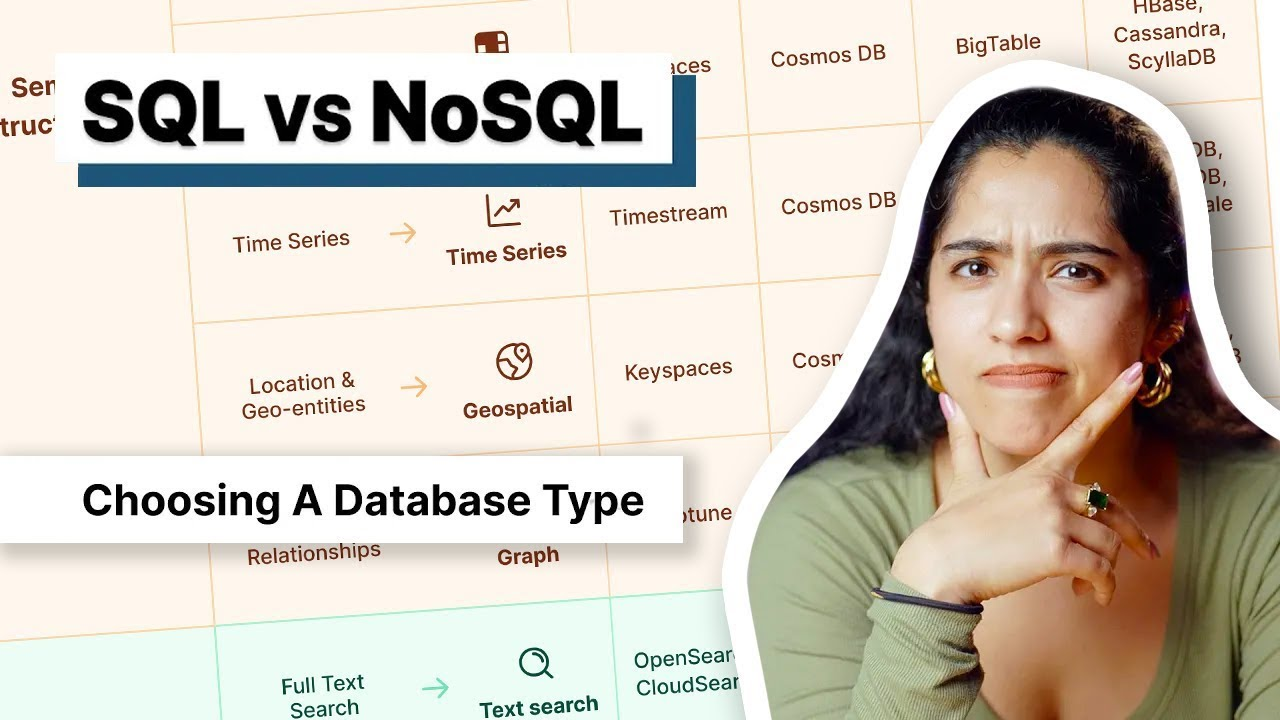
\includegraphics[height=5cm]{img/youtube-thumbnail.jpg}}

\end{frame}


\begin{frame}{Relationnel ou NoSQL ?}


    \textbf{Conception d'un système de réseau social}

    On veut gérer une grande volumétrie de publications. La diffusion de posts auprès de plusieurs utilisateurs peut prendre un certain temps.

    \begin{itemize}
        \item Relationnel
        \item \textcolor<2>{kh-green}{\textbf<2>{NoSQL}}
    \end{itemize}

    \note{
        Étant donné que les données des publications seront principalement des données non structurées (texte/images/vidéos) et que l'on aura besoin d'une évolutivité horizontale (des milliards de publications), on devrait opter pour une base de données NoSQL.
    }

\end{frame}

\begin{frame}{Relationnel ou NoSQL ?}

    \textbf{Conception d'un système de paiement}

    Pour ce système bancaire, il est primordial que les transactions reflètent le compte des client$\cdot$es. Le système ne doit pas créer d'incohérences, ce qui peut entraîner des conséquences indésirables (soldes négatifs) et des client$\cdot$es mécontents.

    \begin{itemize}
        \item \textcolor<2>{kh-green}{\textbf<2>{Relationnel}}
        \item NoSQL
    \end{itemize}

    \note{
        Étant donné que les données sont structurées et que plusieurs utilisateurs n'ont pas besoin de consulter une seule transaction, il est préférable d'utiliser une base de données relationnelle.
    }


\end{frame}
